%& C:\Users\hari\AppData\Roaming\TikzEdt\TikzEdt\021~1.0\TEMP_H~1
\begin{document}

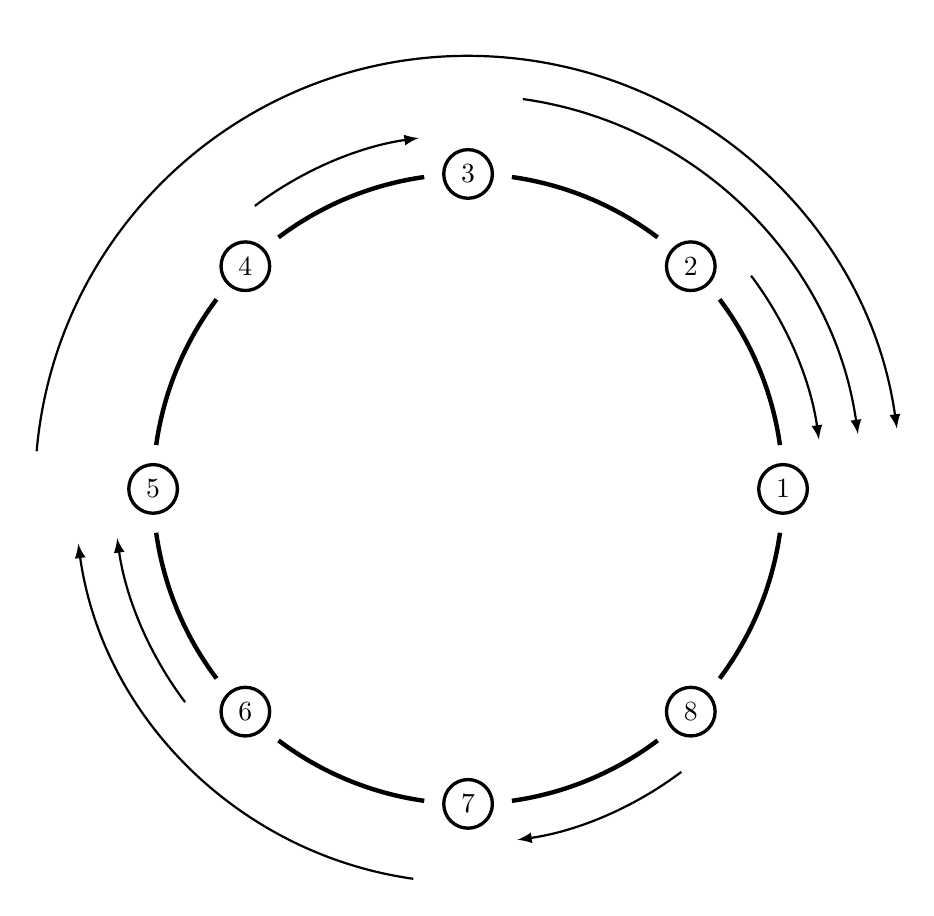
\begin{tikzpicture}

\def \n {8}
\def \radius {4cm}
\def \rone {4.5cm}
\def \rtwo {5cm}
\def \rthr {5.5cm}

\def \margin {8} % margin in angles, depends on the radius

\foreach \s in {1,...,\n}
{
  \node[draw, very thick, circle] at ({360/\n * (\s - 1)}:\radius) {$\s$};
  \draw[ultra thick] ({360/\n * (\s - 1)+\margin}:\radius) 
    arc ({360/\n * (\s - 1)+\margin}:{360/\n * (\s)-\margin}:\radius);
}
\foreach \s in {1,3,...,\n}
{
   \draw[<-, >=latex, thick] ({360/\n * (\s - 1)+\margin}:\rone) 
    arc ({360/\n * (\s - 1)+\margin}:{360/\n * (\s)-\margin}:\rone);
}

\foreach \s in {2,6}
{
   \draw[<-, >=latex, thick] ({360/\n * (\s - 2)+\margin}:\rtwo) 
    arc ({360/\n * (\s - 2)+\margin}:{360/\n * (\s)-\margin}:\rtwo);
}

\draw[->, >=latex, thick] (175:\rthr) arc (175:8:\rthr);


\usetikzlibrary{calc}
\pgftransformreset
\node[inner sep=0pt,outer sep=0pt,minimum size=0pt,line width=0pt,text width=0pt,text height=0pt] at (current bounding box) {};
%add border to avoid cropping by pdflibnet
\foreach \border in {0.1}
  \useasboundingbox (current bounding box.south west)+(-\border,-\border) rectangle (current bounding box.north east)+(\border,\border);
\newwrite\metadatafile
\immediate\openout\metadatafile=\jobname_BB.txt
\path
  let
    \p1=(current bounding box.south west),
    \p2=(current bounding box.north east)
  in
  node[inner sep=0pt,outer sep=0pt,minimum size=0pt,line width=0pt,text width=0pt,text height=0pt,draw=white] at (current bounding box) {
\immediate\write\metadatafile{\p1,\p2}
};
\immediate\closeout\metadatafile
\end{tikzpicture}

\end{document}
